\documentclass[border=5pt]{standalone}
\usepackage{tkz-euclide}
\usetikzlibrary{patterns}
\usepackage{fourier}
\makeatletter
\tikzset{
  invertdim/.style args={#1,#2,#3,#4}{%
    postaction={
      decoration={
        show path construction,
        lineto code={
          \coordinate (tkzInvertDimStart) at ($ (\tikzinputsegmentfirst)!#2!90:(\tikzinputsegmentlast) $);
          \coordinate (tkzInvertDimEnd) at ($ (\tikzinputsegmentlast)!#2!-90:(\tikzinputsegmentfirst) $);
          \coordinate (tkzInvertDimLeftOuter) at ($ (tkzInvertDimStart)!-#4!(tkzInvertDimEnd) $);
          \coordinate (tkzInvertDimRightOuter) at ($ (tkzInvertDimEnd)!-#4!(tkzInvertDimStart) $);
          \draw[invertdim fence style/.try]
            (\tikzinputsegmentfirst) -- ($ (\tikzinputsegmentfirst)!1.25*(#2)!90:(\tikzinputsegmentlast) $)
            (\tikzinputsegmentlast) -- ($ (\tikzinputsegmentlast)!1.25*(#2)!-90:(\tikzinputsegmentfirst) $);
          \path
            ($ (tkzInvertDimStart)!0.5!(tkzInvertDimEnd) $)
            node[inner sep=0pt, font=\footnotesize, fill=\tkz@fillcolor, #3] (tkzInvertDimLabel) {#1};
          \draw[invertdim style/.try] (tkzInvertDimLeftOuter) -- (tkzInvertDimStart);
          \draw[invertdim style/.try] (tkzInvertDimRightOuter) -- (tkzInvertDimEnd);
        }
      },
      decorate,
    }
  },
  invertdim/.default={,0pt,,6pt},
  invertdim style/.style={thick,-latex},
  invertdim fence style/.style={thick},
}
\makeatother
\begin{document}
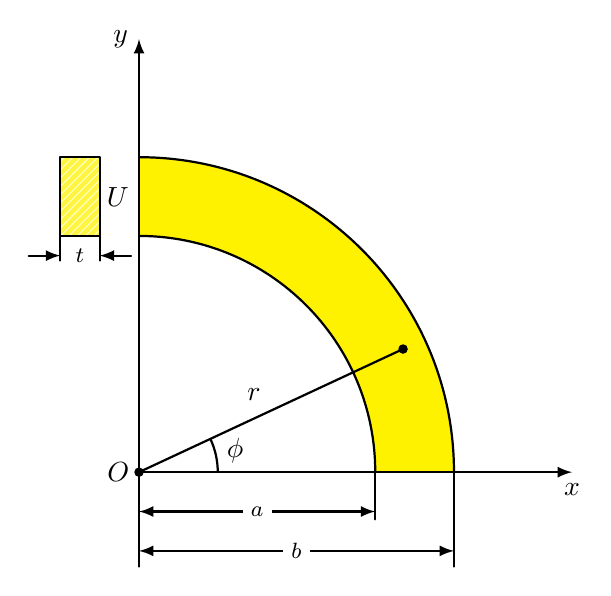
\begin{tikzpicture}[>=latex]
\tkzSetUpLine[line width=.8pt]
\tkzInit[xmax=5,ymin=-1.,ymax=5]
\tkzDefPoints{0/0/O, 4/0/A, 0/4/B, 3/0/A1, 0/3/B1, -.5/3/A2,-1/4/C2}
\tkzDefRectangle(A2,C2)\tkzGetPoints{B2}{D2}
\tkzDrawPolygon[black,preaction={fill,yellow!75},pattern=north east lines,pattern color=yellow!25](A2,B2,C2,D2)
\tkzLabelPoint[left](O){$O$}
\tkzFillSector[yellow](O,A)(B)
\tkzFillSector[white](O,A1)(B1)
\tkzDrawArc[thick](O,A)(B)
\tkzDrawArc[thick](O,A1)(B1)
\tkzDefPoint(25:3.7){P}
\tkzDrawPoints[fill=black,size=3pt](O,P)
\tkzDrawSegment[thick](O,P)
\tkzLabelSegment[above left](O,P){$r$}
\tkzDrawX[thick]\tkzDrawY[thick]
\tkzDrawSegment[dim={$a$,-.5cm,inner xsep=3pt}](O,A1)
\tkzDrawSegment[dim={$b$,-1cm,inner xsep=3pt}](O,A)
\tkzDrawSegment[invertdim={$t$,.25cm,inner xsep=3pt,.4cm}](A2,B2)
\tkzMarkAngle[thick](A,O,P)\tkzLabelAngle[pos=1.25](A,O,P){$\phi$}
\tkzLabelSegment[left](B,B1){$U$}
\end{tikzpicture}
\end{document}
